\vbox{%
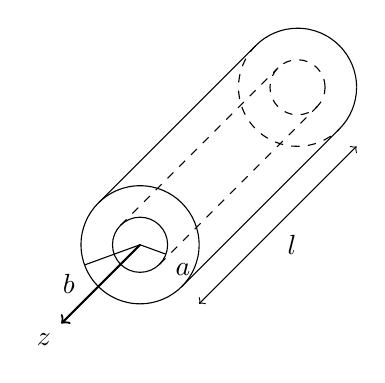
\begin{tikzpicture}
	% Achsen zeichnen
	\draw[->,thick] (0,0) -- (-1,-1) node [below left] {$z$};
	%Plot
	\draw (0,0) circle (.35);
	\draw (0,0) circle (.75);
	\draw (0,0) -- (340:.35) node [below right] {$a$};
	\draw (0,0) -- (200:.75) node[below left] {$b$};
	\draw (135:.75) --+ (2,2);
	\draw[style=dashed] (135:.35) --+ (2,2);
	\draw[style=dashed] (315:.35) --+ (2,2);
	\draw (315:.75) --+ (2,2);
	\draw[style=dashed] (2,2) circle (.35);
	\draw (2,2) +(0:.75) arc (0:135:0.75) ;
	\draw[style=dashed] (2,2)+(135:.75) arc (135:315:.75);
	\draw (2,2) +(315:.75) arc (315:360:.75);
	\draw[<-] (.75,-0.75)--(1.75,0.25) node[below right] {$l$};
	\draw[->] (1.75,0.25)--(2.75,1.25);
      \end{tikzpicture}
      
\begin{tikzpicture}
	% Achsen zeichnen
	%\draw[->,thick] (0,0) -- (-1,-1) node [below left] {$z$};
	\draw[<->] (0,0)--(0,2) node[left] {$2b$} --(0,4);
	\draw[<->] (1,1.5)--(1,2) node[left] {$2a$} --(1,2.5);
	\draw (1.5,4)--(5.5,4);
	\draw (1.5,0)--(5.5,0)--(5.5,2);
	\draw[->] (1.5,2)--(7,2) node[right] {$z$};
	\draw (1.5,0)--(1.5,2);
	\draw (1.5,1) circle(.25);
	\draw[<-] (1.1,.75)--(1.1,1.25) node[below left] {$\spannung_0$};	
	\draw (1.9,1.5) rectangle (5,2.5);
	\draw[style=dashed] (1.9,2.5)--(1.9,4.2) node[above] {$0$};
	\draw[style=dashed] (3.5,2.5)--(3.5,4.2) node[above] {$z$};
	\draw[fill=black] (1.7,0) circle(.05);
	\draw[fill=black] (1.7,2) circle(.05);
	\draw[fill=black] (5.3,0) circle(.05);
	\draw[fill=black] (5.3,2) circle(.05);
	\draw[fill=white] (5.35,0.5) rectangle (5.65,1.5);
	\node[right] at (5.75,1) {$\elwiderstand$};
	\node[right] at (3,1.65) {$\kappa$};
	\node[right] at (3,-.3) {$\kappa_a \rightarrow \infty$};
	\node[right] at (3.2,.75) {$\spannung ( z)$};
	\draw[->] (3.2,1.3)--(3.2,0.2);
      \end{tikzpicture}
}